% Source: graduate-coursework/Research/Intro_to_Agents/handouts/Part6_MultiTier_Architecture.tex

\documentclass[border=4pt]{standalone}
\usepackage{amsmath,amssymb,amsfonts}
\usepackage[T1]{fontenc}
\usepackage{graphicx}
\usepackage{lmodern}
\usepackage{tikz}
\usepackage{xcolor}
\usetikzlibrary{shapes,arrows.meta,positioning,calc,fit,backgrounds,chains,decorations.pathreplacing}

\definecolor{UofSCGarnet}{HTML}{73000a}
\definecolor{UofSCBlack}{HTML}{000000}
\definecolor{UofSCWhite}{HTML}{ffffff}
\definecolor{UofSCRose}{HTML}{CC2E40}
\definecolor{UofSCAtlantic}{HTML}{466A9F}
\definecolor{UofSCCongaree}{HTML}{1F414D}
\definecolor{UofSCHorseshoe}{HTML}{65780B}
\definecolor{UofSCGrass}{HTML}{CED318}
\definecolor{UofSCHoneycomb}{HTML}{A49137}
\definecolor{UofSC90Black}{HTML}{363636}
\definecolor{UofSC70Black}{HTML}{5C5C5C}
\definecolor{UofSC50Black}{HTML}{A2A2A2}
\definecolor{UofSCWarmGrey}{HTML}{676156}
\definecolor{UofSCSandstorm}{HTML}{FFF2E3}
\definecolor{UofSCDarkGarnet}{HTML}{570008}
\definecolor{UofSCAzalea}{HTML}{844247}

\tikzset{
    % Base node style
    basenode/.style={
        draw=UofSCBlack,
        fill=UofSCWhite,
        line width=0.8pt,
        minimum height=0.8cm,
        minimum width=2cm,
        align=center,
        font=\small
    },
    % Strategy layer style
    strategynode/.style={
        basenode,
        fill=UofSCGarnet,
        text=UofSCWhite,
        minimum height=1cm,
        minimum width=4cm
    },
    % Planning layer style
    planningnode/.style={
        basenode,
        fill=UofSCAtlantic,
        text=UofSCWhite,
        minimum height=0.9cm,
        minimum width=3.5cm
    },
    % Execution layer style
    execnode/.style={
        basenode,
        fill=UofSCCongaree,
        text=UofSCWhite,
        minimum height=0.8cm,
        minimum width=2.5cm
    },
    % Generic box
    genericbox/.style={
        basenode,
        minimum width=2.8cm
    },
    % Arrow styles (straight lines only)
    myarrow/.style={
        ->,
        >=Stealth,
        line width=0.8pt,
        draw=UofSCBlack
    },
    % Bidirectional arrow
    biarrow/.style={
        <->,
        >=Stealth,
        line width=0.8pt,
        draw=UofSCBlack
    },
    % Phase box style
    phasebox/.style={
        basenode,
        minimum width=3.5cm,
        minimum height=1.2cm,
        font=\small\bfseries
    },
    % Small box
    smallbox/.style={
        basenode,
        minimum width=1.5cm,
        minimum height=0.6cm,
        font=\scriptsize
    },
    % Leader node
    leadernode/.style={
        basenode,
        fill=UofSCGarnet,
        text=UofSCWhite,
        minimum width=3cm,
        minimum height=1cm
    },
    % Worker node
    workernode/.style={
        basenode,
        fill=UofSC70Black,
        text=UofSCWhite,
        minimum width=1.2cm,
        minimum height=0.7cm,
        font=\scriptsize
    }
}

\begin{document}
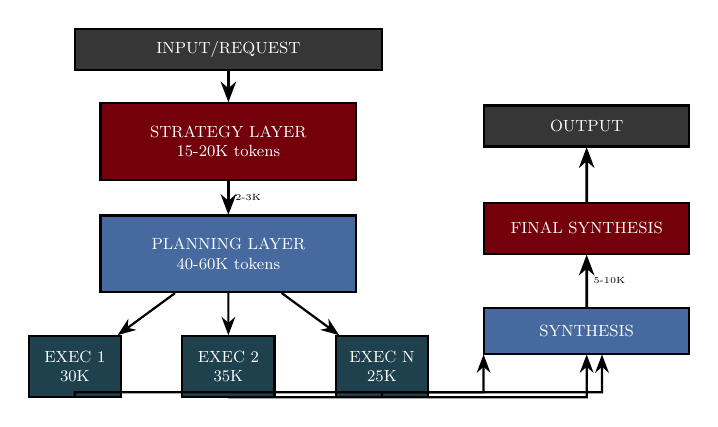
\begin{tikzpicture}[scale=0.65, transform shape]
        % Input
        \node[genericbox, fill=UofSC90Black, text=white, minimum width=6cm] (input) at (0,7) {INPUT/REQUEST};

        % Strategy
        \node[strategynode, minimum width=5cm, minimum height=1.5cm] (strat) at (0,5.2) {STRATEGY LAYER\\15-20K tokens};

        % Planning
        \node[planningnode, minimum width=5cm, minimum height=1.5cm] (plan) at (0,3) {PLANNING LAYER\\40-60K tokens};

        % Execution agents
        \node[execnode, minimum width=1.8cm, minimum height=1.2cm] (exec1) at (-3,0.8) {EXEC 1\\30K};
        \node[execnode, minimum width=1.8cm, minimum height=1.2cm] (exec2) at (0,0.8) {EXEC 2\\35K};
        \node[execnode, minimum width=1.8cm, minimum height=1.2cm] (exec3) at (3,0.8) {EXEC N\\25K};

        % Synthesis
        \node[planningnode, minimum width=4cm] (synth) at (7,1.5) {SYNTHESIS};
        \node[strategynode, minimum width=4cm] (final) at (7,3.5) {FINAL SYNTHESIS};

        % Output
        \node[genericbox, fill=UofSC90Black, text=white, minimum width=4cm] (output) at (7,5.5) {OUTPUT};

        % Arrows
        \draw[myarrow, line width=1pt] (input) -- (strat);
        \draw[myarrow, line width=1pt] (strat) -- node[right,font=\tiny]{2-3K} (plan);
        \draw[myarrow] (plan) -- (exec1);
        \draw[myarrow] (plan) -- (exec2);
        \draw[myarrow] (plan) -- (exec3);

        \draw[myarrow] (exec1) -- ++(0,-0.5) -| (synth.south west);
        \draw[myarrow] (exec2) -- ++(0,-0.6) -| (synth.south);
        \draw[myarrow] (exec3) -- ++(0,-0.5) -| ($(synth.south)+(0.3,0)$);

        \draw[myarrow, line width=1pt] (synth) -- node[right,font=\tiny]{5-10K} (final);
        \draw[myarrow, line width=1pt] (final) -- (output);
    \end{tikzpicture}
\end{document}
